\chapter{Loops and strings}

Computers are often used to automate repetitive tasks, such as searching for text in documents.
Repeating tasks without making errors is something that computers do well and people do poorly.

In this chapter, we'll learn how to use \java{while} and \java{for} loops to add repetition to your code.
We'll also take a first look at \java{String} methods and solve some interesting problems.

%We have seen methods, like \java{countdown} and \java{factorial}, that use recursion to iterate.
%Although recursion is elegant and powerful, it takes some getting used to.
%Java provides language features that make iteration much easier: the \java{while} and \java{for} statements.


\section{The while statement}

\index{while}
\index{loop!while}
\index{statement!while}

Using a \java{while} statement, we can repeat the same code multiple times:

\begin{code}
int n = 3;
while (n > 0) {
    System.out.println(n);
    n = n - 1;
}
System.out.println("Blastoff!");
\end{code}

Reading the code in English sounds like: ``Start with \java{n} set to 3.
While \java{n} is greater than zero, print the value of \java{n}, and reduce the value of \java{n} by 1.
When you get to zero, print Blastoff!''
So the output is:

\begin{stdout}
3
2
1
Blastoff!
\end{stdout}

The flow of execution for a \java{while} statement is:

\begin{enumerate}

\item Evaluate the condition in parentheses, yielding \java{true} or \java{false}.

\item If the condition is \java{false}, skip the following statements in braces.

\item If the condition is \java{true}, execute the statements and go back to step 1.

\end{enumerate}

\index{loop}

This type of flow is called a {\bf loop}, because the last step ``loops back around'' to the first.
Figure~\ref{fig.while} shows this idea using a flowchart.

\begin{figure}[!ht]
\begin{center}
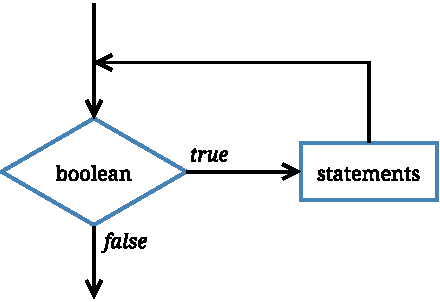
\includegraphics[scale=0.9]{figs/while.pdf}
\caption{Flow of execution for a \java{while} loop.}
\label{fig.while}
\end{center}
\end{figure}

\index{loop body}
\index{infinite loop}
\index{loop!infinite}

The {\bf body} of the loop should change the value of one or more variables so that, eventually, the condition becomes \java{false} and the loop terminates.
Otherwise the loop will repeat forever, which is called an {\bf infinite loop}.

\begin{code}
int n = 3;
while (n > 0) {
    System.out.println(n);
    // n never changes
}
\end{code}

This example will print the number \java{3} forever, or at least until you terminate the program.
An endless source of amusement for computer scientists is the observation that the directions on shampoo, ``Lather, rinse, repeat,'' are an infinite loop.

In the first example, we can prove that the loop terminates when \java{n} is positive.
But in general, it is not so easy to tell whether a loop terminates.
For example, this loop continues until \java{n} is 1 (which makes the condition \java{false}):

\begin{code}
while (n != 1) {
    System.out.println(n);
    if (n % 2 == 0) {         // n is even
        n = n / 2;
    } else {                  // n is odd
        n = 3 * n + 1;
    }
}
\end{code}

Each time through the loop, the program displays the value of \java{n} and then checks whether it is even or odd.
If it is even, the value of \java{n} is divided by two.
If it is odd, the value is replaced by $3n+1$.
For example, if the starting value is 3, the resulting sequence is 3, 10, 5, 16, 8, 4, 2, 1.

Since \java{n} sometimes increases and sometimes decreases, there is no obvious proof that \java{n} will ever reach 1 and that the program will ever terminate.
For some values of \java{n}, such as the powers of two, we can prove that it terminates.
The previous example ends with such a sequence, starting when \java{n} is 16 (or $2^4$).

The hard question is whether this program terminates for {\em all} values of n.
So far, no one has been able to prove it {\em or} disprove it!
For more information, see \url{https://en.wikipedia.org/wiki/Collatz_conjecture}.
%The field of computer science is interested in these types of questions, because their answers give insight to the limits of what computers can and cannot do.


\section{Increment and decrement}

Here is another \java{while} loop example; this one displays the numbers 1 to 5.

\begin{code}
int i = 1;
while (i <= 5) {
    System.out.println(i);
    i++;  // add 1 to i
}
\end{code}

\index{increment}
\index{decrement}

Assignments like \java{i = i + 1} don't often appear in loops, because Java provides a more concise way to add and subtract by one.
Specifically, \java{++} is the {\bf increment} operator; it has the same effect as \java{i = i + 1}.
And \java{--} is the {\bf decrement} operator; it has the same effect as \java{i = i - 1}.

%So far in this book we have only used (\java{=}) to assign values to variables.
%For convenience, Java provides other assignment operators that increase or decrease the value of a variable.

If you want to increment or decrement a variable by an amount other than \java{1}, you can use \java{+=} and \java{-=}.
For example, \java{i += 2} increments \java{i} by \java{2}.

\begin{code}
int i = 2;
while (i <= 8) {
    System.out.print(i + ", ");
    i += 2;  // add 2 to i
}
System.out.println("Who do we appreciate?");
\end{code}

And the output is:

\begin{stdout}
2, 4, 6, 8, Who do we appreciate?
\end{stdout}


\section{The for statement}

\index{for}
\index{loop!for}
\index{statement!for}

The loops we have written so far have several elements in common.
They start by initializing a variable, they have a condition that depends on that variable, and inside the loop they do something to update that variable.

\index{iteration}

Running the same code multiple times is called {\bf iteration}.
This type of loop is so common that there is another statement, the \java{for} loop, that expresses it more concisely.
For example, we can rewrite the 2-4-6-8 loop this way:

\begin{code}
for (int i = 2; i <= 8; i += 2) {
    System.out.print(i + ", ");
}
System.out.println("Who do we appreciate?");
\end{code}

\java{for} loops have three components in parentheses, separated by semicolons: the initializer, the condition, and the update.

\begin{enumerate}

\item The {\em initializer} runs once at the very beginning of the loop.
(It is equivalent to the line before the \java{while} statement.)

\item The {\em condition} is checked each time through the loop.
If it is \java{false}, the loop ends.
Otherwise, the body of the loop is executed (again).

\item At the end of each iteration, the {\em update} runs, and we go back to step~2.

\end{enumerate}

The \java{for} loop is often easier to read because it puts all the loop-related statements at the top of the loop.
Doing so allows you to focus on the statements in the loop body.
Figure~\ref{fig.for} illustrates \java{for} loops with a flowchart.

\begin{figure}[!ht]
\begin{center}
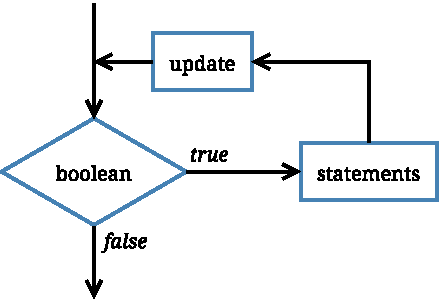
\includegraphics[scale=0.9]{figs/for.pdf}
\caption{Flow of execution for a \java{for} loop.}
\label{fig.for}
\end{center}
\end{figure}

There is another difference between \java{for} loops and \java{while} loops: if you declare a variable in the initializer, it only exists {\em inside} the \java{for} loop.
For example:

\begin{code}
for (int n = 3; n > 0; n--) {
    System.out.println(n);
}
System.out.println("n is now " + n);  // compiler error
\end{code}

The last line tries to display \java{n} (for no reason other than demonstration) but it won't work.
If you need to use a loop variable outside the loop, you have to declare it {\em outside} the loop, like this:

\begin{code}
int n;
for (n = 3; n > 0; n--) {
    System.out.println(n);
}
System.out.println("n is now " + n);
\end{code}

Notice that the \java{for} statement does not say \java{int n = 3}.
Rather, it simply initializes the existing variable \java{n}.


\section{Nested loops}
\label{nested}

\index{loop!nested}
\index{nested!loops}

Like conditional statements, loops can be nested one inside the other.
Nested loops allow you to iterate over two variables.
For example, we can generate a ``multiplication table'' like this:

\begin{code}
for (int x = 1; x <= 10; x++) {
    for (int y = 1; y <= 10; y++) {
        System.out.printf("%4d", x * y);
    }
    System.out.println();
}
\end{code}

\index{loop variable}
\index{variable!loop}
\index{inner loop}
\index{outer loop}

Variables like \java{x} and \java{y} are called {\bf loop variables}, because they control the execution of a loop.
In this example, the first loop (\java{for x}) is known as the ``outer loop'', and the second loop (\java{for y}) is known as the ``inner loop''.

Each loop repeats their corresponding statements 10 times.
The outer loop iterates from 1 to 10 only once, but the inner loop iterates from 1 to 10 each of those 10 times.
As a result, the \java{printf} method is invoked 100 times.

\index{format specifier}

The format specifier \java{\%4d} displays the value of \java{x * y} padded with spaces so it's four characters wide.
Doing so causes the output to align vertically, regardless of how many digits the numbers have:

\begin{stdout}
   1   2   3   4   5   6   7   8   9  10
   2   4   6   8  10  12  14  16  18  20
   3   6   9  12  15  18  21  24  27  30
   4   8  12  16  20  24  28  32  36  40
   5  10  15  20  25  30  35  40  45  50
   6  12  18  24  30  36  42  48  54  60
   7  14  21  28  35  42  49  56  63  70
   8  16  24  32  40  48  56  64  72  80
   9  18  27  36  45  54  63  72  81  90
  10  20  30  40  50  60  70  80  90 100
\end{stdout}

It's important to realize that the output is displayed row by row.
The inner loop displays a single row of output, followed by a newline.
The outer loop iterates over the rows themselves.
Another way to read nested loops, like the ones in this example, is ``for each row \java{x}, and for each column \java{y}, \ldots''


\section{Characters}

Some of the most interesting problems in computer science involve searching and manipulating text.
In the next few sections, we'll discuss how to apply loops to strings.
Although the examples are short, the techniques work the same whether you have one word or one million words.

\index{charAt}
\index{char}
\index{type!char}

Strings provide a method named \java{charAt}.
It returns a \java{char}, a data type that stores an individual character (as opposed to strings of them).

\begin{code}
String fruit = "banana";
char letter = fruit.charAt(0);
\end{code}

The argument \java{0} means that we want the character at {\bf index} 0.
String indexes range from 0 to $n-1$, where $n$ is the length of the string.
So the character assigned to \java{letter} is \java{b}.

\begin{center}
\ttfamily
\begin{tabular}{cccccc}
\hline
\multicolumn{1}{|l|}{b} & \multicolumn{1}{l|}{a} & \multicolumn{1}{l|}{n} & \multicolumn{1}{l|}{a} & \multicolumn{1}{l|}{n} & \multicolumn{1}{l|}{a} \\ \hline
0                       & 1                      & 2                      & 3                      & 4                      & 5
\end{tabular}
\end{center}


Characters work like the other data types we have seen.
You can compare them using relational operators:

\begin{code}
if (letter == 'a') {
    System.out.println('?');
}
\end{code}

\index{quote mark}
\index{escape sequence}

Character literals, like \java{'a'}, appear in single quotes.
Unlike string literals, which appear in double quotes, character literals can only contain a single character.
Escape sequences, like \java{'\\t'}, are legal because they represent a single character.

The increment and decrement operators also work with characters.
So this loop displays the letters of the alphabet:

\begin{code}
System.out.print("Roman alphabet: ");
for (char c = 'A'; c <= 'Z'; c++) {
    System.out.print(c);
}
System.out.println();
\end{code}

\index{Unicode}

Java uses {\bf Unicode} to represent characters, so strings can store text in other alphabets like Cyrillic and Greek, and non-alphabetic languages like Chinese.
You can read more about it at \url{http://unicode.org/}.

In Unicode, each character is represented by a ``code point'', which you can think of as an integer.
The code points for uppercase Greek letters run from 913 to 937, so we can display the Greek alphabet like this:

\begin{code}
System.out.print("Greek alphabet: ");
for (int i = 913; i <= 937; i++) {
    System.out.print((char) i);
}
System.out.println();
\end{code}

This example uses a type cast to convert each integer (in the range) to the corresponding character.
Try running the code and see what happens.


\section{String iteration}

\index{iteration}

The following loop iterates the characters in \java{fruit} and displays them, one on each line:

\begin{code}
for (int i = 0; i < fruit.length(); i++) {
    char letter = fruit.charAt(i);
    System.out.println(letter);
}
\end{code}

\index{string!length}
\index{length!string}

Strings provide a method called \java{length} that returns the number of characters in the string.
Because it is a method, you have to invoke it with the empty argument list, \java{()}.
When \java{i} is equal to the length of the string, the condition becomes \java{false} and the loop terminates.

To find the last letter of a string, you might be tempted to do something like:

\begin{code}
int length = fruit.length();
char last = fruit.charAt(length);      // wrong!
\end{code}

\index{StringIndexOutOfBoundsException}
\index{exception!StringIndexOutOfBounds}

This code compiles and runs, but invoking the \java{charAt} method throws a \java{StringIndexOutOfBoundsException}.
The problem is that there is no sixth letter in \java{"banana"}.
Since we started counting at 0, the 6 letters are indexed from 0 to 5.
To get the last character, you have to subtract 1 from \java{length}.

\begin{code}
int length = fruit.length();
char last = fruit.charAt(length - 1);  // correct
\end{code}

Many string algorithms involve reading one string and building another.
For example, to reverse a string, we can add one character at a time:

\begin{code}
public static String reverse(String s) {
    String r = "";
    for (int i = s.length() - 1; i >= 0; i--) {
        r += s.charAt(i);
    }
    return r;
}
\end{code}

\index{empty string}

The initial value of \java{r} is \java{""}, which is the {\bf empty string}.
The loop iterates the letters of \java{s} in reverse order.
Each time through the loop, it creates a new string and assigns it to \java{r}.
When the loop exits, \java{r} contains the letters from \java{s} in reverse order.
So the result of \java{reverse("banana")} is \java{"ananab"}.


\section{The indexOf method}

\index{indexOf}

To search for a specific character in a string, you could write a \java{for} loop and use \java{charAt} like in the previous section.
However, the \java{String} class already provides a method for doing just that.

\begin{code}
String fruit = "banana";
int index = fruit.indexOf('a');     // returns 1
\end{code}

This example finds the index of \java{'a'} in the string.
But the letter appears three times, so it's not obvious what \java{indexOf} should do.
According to the documentation, it returns the index of the {\em first} appearance.

To find subsequent appearances, you can use another version of \java{indexOf}, which takes a second argument that indicates where in the string to start looking.

\begin{code}
int index = fruit.indexOf('a', 2);  // returns 3
\end{code}

To visualize how \java{indexOf} and other \java{String} methods work, it helps to draw a picture like Figure~\ref{fig.banana}.
The previous code starts at index 2 (the first \java{'n'}) and finds the next \java{'a'}, which is at index 3.

\index{memory diagram}
\index{diagram!memory}

\begin{figure}[!ht]
\begin{center}
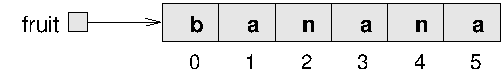
\includegraphics{figs/banana.pdf}
\caption{Memory diagram for a \java{String} of six characters.}
\label{fig.banana}
\end{center}
\end{figure}

%\begin{center}
%\begin{tabular}{c|c|c|c|c|c}
%%\hline
%b & a & n & a & n & a \\
%\hline
%0 & 1 & 2 & 3 & 4 & 5 \\
%%\hline
%\end{tabular}
%\end{center}

If the character happens to appear at the starting index, the starting index is the answer.
So \java{fruit.indexOf('a', 5)} returns \java{5}.
If the character does not appear in the string, \java{indexOf} returns \java{-1}.
Since indexes cannot be negative, this value indicates the character was not found.

You can also use \java{indexOf} to search for an entire string, not just a single character.
For example, the expression \java{fruit.indexOf("nan")} returns \java{2}.


\section{String comparison}
\label{strcmp}

\index{equals}
\index{string!comparing}

To compare two strings, it may be tempting to use the \java{==} and \java{!=} operators.

\begin{code}
String name1 = "Alan Turing";
String name2 = "Ada Lovelace";
if (name1 == name2) {                 // wrong!
    System.out.println("The names are the same.");
}
\end{code}

This code compiles and runs, and sometimes it gets the answer right.
But sometimes it gets the answer wrong.
If you give it two different strings that contain the same letters, the condition will be \java{false}.

The problem is that the \java{==} operator checks whether the two variables refer to the {\em same object} by comparing the references.
We'll learn more about references in the next chapter.
The correct way to compare strings is with the \java{equals} method, like this:

\begin{code}
if (name1.equals(name2)) {
    System.out.println("The names are the same.");
}
\end{code}

This example invokes \java{equals} on \java{name1} and passes \java{name2} as an argument.
The \java{equals} method returns \java{true} if the strings contain the same characters; otherwise it returns \java{false}.

\index{compareTo}

If the strings differ, we can use \java{compareTo} to see which comes first in alphabetical order:

\begin{code}
int diff = name1.compareTo(name2);
if (diff == 0) {
    System.out.println("The names are the same.");
} else if (diff < 0) {
    System.out.println("name1 comes before name2.");
} else if (diff > 0) {
    System.out.println("name2 comes before name1.");
}
\end{code}

The return value from \java{compareTo} is the difference between the first characters in the strings that are not the same.
In the preceding code, \java{compareTo} returns positive 8, because the second letter of \java{"Ada"} comes before the second letter of \java{"Alan"} by 8 letters.

If the strings are equal, their difference is zero.
If the first string (the one on which the method is invoked) comes first in the alphabet, the difference is negative.
Otherwise, the difference is positive.

\index{case-sensitive}

Both \java{equals} and \java{compareTo} are case-sensitive.
In Unicode, uppercase letters come before lowercase letters.
So \java{"Ada"} comes before \java{"ada"}.


\section{Substrings}

\index{substring}

The \java{substring} method returns a new string that copies letters from an existing string, starting at the given index.

\begin{itemize}
\item \java{fruit.substring(0)} returns \java{"banana"}
\item \java{fruit.substring(2)} returns \java{"nana"}
\item \java{fruit.substring(6)} returns \java{""}
\end{itemize}

The first example returns a copy of the entire string.
The second example returns all but the first two characters.
As the last example shows, \java{substring} returns the empty string if the argument is the length of the string.

Like most string methods, \java{substring} is overloaded.
That is, there are other versions of \java{substring} that have different parameters.
If it's invoked with two arguments, they are treated as a start and end index:

\begin{itemize}
\item \java{fruit.substring(0, 3)} returns \java{"ban"}
\item \java{fruit.substring(2, 5)} returns \java{"nan"}
\item \java{fruit.substring(6, 6)} returns \java{""}
\end{itemize}

Notice that the character indicated by the end index is {\em not} included.
Defining \java{substring} this way simplifies some common operations.
For example, to select a substring with length \java{len}, starting at index \java{i}, you could write \java{fruit.substring(i, i + len)}.
%So \java{fruit.substring(2, 2 + 3)} returns \java{"nan"}.


\section{String formatting}

\index{printf}

In Section~\ref{printf}, we learned how to use \java{System.out.printf} to display formatted output.
Sometimes programs need to create strings that are formatted a certain way, but not display them immediately, or ever.
For example, the following method returns a time string in 12-hour format:

\begin{code}
public static String timeString(int hour, int minute) {
    String ampm;
    if (hour < 12) {
        ampm = "AM";
        if (hour == 0) {
            hour = 12;  // midnight
        }
    } else {
        ampm = "PM";
        hour = hour - 12;
    }
    return String.format("%02d:%02d %s", hour, minute, ampm);
}
\end{code}

\index{string!format}

\java{String.format} takes the same arguments as \java{System.out.printf}: a format specifier followed by a sequence of values.
The main difference is that \java{System.out.printf} displays the result on the screen.
\java{String.format} creates a new string, but does not display anything.

In this example, the format specifier \java{\%02d} means ``two digit integer padded with zeros'', so \java{timeString(19, 5)} returns the string \java{"07:05 PM"}.
As an exercise, try writing two nested \java{for} loops (in \java{main}) that invoke \java{timeString} and display all possible times over a 24-hour period.

At some point today, skim through the documentation for \java{String}.
Knowing what other methods are there will help you avoid reinventing the wheel.
The easiest way to find documentation for Java classes is to do a web search for ``Java'' and the name of the class.


\section{Vocabulary}

\begin{description}

\term{loop}
A statement that executes a sequence of statements repeatedly.

\term{loop body}
The statements inside the loop.

\term{infinite loop}
A loop whose condition is always true.

\term{increment}
Increase the value of a variable.

\term{decrement}
Decrease the value of a variable.

\term{iteration}
Executing a sequence of statements repeatedly.

\term{loop variable}
A variable that is initialized, tested, and updated in order to control a loop.

\term{index}
An integer variable or value used to indicate a character in a string.

\term{Unicode}
An international standard for representing characters in most of the world's languages.

\term{empty string}
The string \java{""}, which contains no characters and has a length of zero.

\end{description}


\section{Exercises}

The code for this chapter is in the {\tt ch06} directory of {\tt ThinkJavaCode2}.
See page~\pageref{code} for instructions on how to download the repository.
Before you start the exercises, we recommend that you compile and run the examples.

If you have not already read Appendix~\ref{debugger}, now might be a good time.
It describes the DrJava debugger, which is a useful tool for visualizing the flow of execution through loops.


\begin{exercise}  %%V6 Ex7.1

Consider the following methods:

\begin{code}
public static void main(String[] args) {
    loop(10);
}

public static void loop(int n) {
    int i = n;
    while (i > 1) {
        System.out.println(i);
        if (i % 2 == 0) {
            i = i / 2;
        } else {
            i = i + 1;
        }
    }
}
\end{code}

\begin{enumerate}

\item Draw a table that shows the value of the variables \java{i} and \java{n} during the execution of \java{loop}.
The table should contain one column for each variable and one line for each iteration.

\item What is the output of this program?

\item Can you prove that this loop terminates for any positive value of \java{n}?

% If i is odd and we increment by 1, the result is even.  So the second
% branch is always followed by the first branch.
% If i is even and we divide by 2, the result might be odd.  So in the
% worst case, we might alternate between the branches.
% But we can't do more of the second branch than the first.
% So we divide at least as often as we add.

% If i is 1, we're done.
% If i is 2, we divide by 2 and we're done.
% If i is greater than 2, the first branch decreases more than the
% second branch increases.
% So if we do one of each, the net effect is a decrease.
% Therefore, the value of i has to decrease after any two steps.

\end{enumerate}

\end{exercise}


\begin{exercise}  %%V6 Ex7.2

Let's say you are given a number, $a$, and you want to find its square root.
One way to do that is to start with a rough guess about the answer, $x_0$, and then improve the guess using this formula:
%
\[ x_1 =(x_0 + a/x_0) / 2 \]
%
For example, if we want to find the square root of 9, and we start with $x_0 = 6$, then $x_1 = (6 + 9/6) / 2 = 3.75$, which is closer.
We can repeat the procedure, using $x_1$ to calculate $x_2$, and so on.
In this case, $x_2 = 3.075$ and $x_3 = 3.00091$.
So it converges quickly on the correct answer.

Write a method called \java{squareRoot} that takes a \java{double} and returns an approximation of the square root of the parameter, using this technique.
You should not use \java{Math.sqrt}.

As your initial guess, you should use $a/2$.
Your method should iterate until it gets two consecutive estimates that differ by less than 0.0001.
%In other words, return when the absolute value of $x_n - x_{n-1}$ is less than 0.0001.
You can use \java{Math.abs} to calculate the absolute value of the difference.

\end{exercise}


\begin{exercise}  %%V6 Ex7.6

One way to evaluate $\exp(-x^2)$ is to use the infinite series expansion:
%
\[ \exp(-x^2) = 1 - x^2 + x^4/2 - x^6/6 + \ldots \]
%
The $i$th term in this series is $(-1)^i x^{2i} / i!$.
Write a method named \java{gauss} that takes \java{x} and \java{n} as arguments and returns the sum of the first \java{n} terms of the series.
You should not use \java{factorial} or \java{pow}.

\end{exercise}


\begin{exercise}  %%V6 Ex9.5

\index{abecedarian}

A word is said to be ``abecedarian'' if the letters in the word appear in alphabetical order.
For example, the following are all six-letter English abecedarian words:

\begin{quote}
abdest, acknow, acorsy, adempt, adipsy, agnosy, befist, behint, %\\
beknow, bijoux, biopsy, cestuy, chintz, deflux, dehors, dehort, %\\
deinos, diluvy, dimpsy %\\
\end{quote}

Write a method called \java{isAbecedarian} that takes a \java{String} and returns a \java{boolean} indicating whether the word is abecedarian.
%Your method can be iterative or recursive.

\end{exercise}


\begin{exercise}  %%V6 Ex9.6
\label{doubloon}

\index{doubloon}

A word is said to be a ``doubloon'' if every letter that appears in the word appears exactly twice.
Here are some example doubloons found in the dictionary:

\begin{quote}
Abba, Anna, appall, appearer, appeases, arraigning, beriberi, bilabial, boob, Caucasus, coco, Dada, deed, Emmett, Hannah, horseshoer, intestines, Isis, mama, Mimi, murmur, noon, Otto, papa, peep, reappear, redder, sees, Shanghaiings, Toto
\end{quote}

Write a method called \java{isDoubloon} that takes a string and checks whether it is a doubloon.
To ignore case, invoke the \java{toLowerCase} method before checking.
\end{exercise}


\begin{exercise}  %%V6 Ex9.8

\index{Scrabble}

In Scrabble\footnote{Scrabble is a registered trademark owned in the USA and Canada by Hasbro Inc., and in the rest of the world by J.\ W.\ Spear \& Sons Limited of Maidenhead, Berkshire, England, a subsidiary of Mattel Inc.} each player has a set of tiles with letters on them.
The object of the game is to use those letters to spell words.
The scoring system is complex, but longer words are usually worth more than shorter words.

Imagine you are given your set of tiles as a string, like \java{"quijibo"}, and you are given another string to test, like \java{"jib"}.

Write a method called \java{canSpell} that takes two strings and checks whether the set of tiles can spell the word.
You might have more than one tile with the same letter, but you can only use each tile once.

\end{exercise}
